\documentclass[a4paper,11pt,english]{article}
\usepackage[T1]{fontenc}
\usepackage[utf8]{inputenc}
\usepackage{lmodern}
\usepackage{graphicx}
\usepackage{babel,blindtext}
\usepackage{float}
\usepackage{wrapfig}	
\title{PH21 Assignment 2}
\author{Helen Xue}

\begin{document}

\maketitle

\begin{enumerate}
	\item 
	\begin{enumerate}
		\item $$\widetilde{h_k} = \frac{1}{L} \int_{0}^{L} h(x)e^{2\pi if_kx}dx$$ $$h(x) = \sum_{k=-\infty}^{\infty} \widetilde{h_k}e^{-2 \pi i f_kx}, f_k = \frac{k}{L}$$
		\par Plugging 2 into 1 
		$$h(x) = \sum_{k=-\infty}^{\infty} [ \frac{1}{L}\int_{0}^{L}h(x')e^{2\pi ikx'/L}dx']e^{-2 \pi i k x/L}$$
		\par We can swap the sum and the integral, pulling out $h(x')$ to get
		$$ h(x) = \int_0^L h(x') \delta(x'-x)dx' = h(x), x' \neq xs$$
		
		\item We use Euler's trig relation, which says $sin(2\pi x/L + \phi) = \frac{e^{-i(2\pi x/L + \phi)}+ e^{-i(2\pi x/L + \phi)}}{2i}$. Pulling out the terms that we want, we get that a linear combination of $e^{-2\pi i x/L}$ and $e^{2\pi i x/L}$ with coefficients $A\frac{e^{\pm i\phi}}{2i}$, which are both constant, can represent any function $Asin(2\pi x/L + \phi)$.
		
		 Since we know that sines and cosines are offset by some phase, we know that this can also represent any cosine function.
		
		\item $\widetilde h_{-k} = \widetilde h_k^*$?
		
		\par $\widetilde h_{-k} = \int_0^L \frac{1}{L} h(x)e^{-2\pi i kx/L}dx $  
		\par $\widetilde h_k^* = [\int_0^L \frac{1}{L} h(x)e^{2\pi i kx/L}dx ]^*$
		\par Since $h(x)$ is real, we can write
		\par $\widetilde h_k^* = \int_0^L \frac{1}{L} h(x)[e^{2\pi i kx/L}dx ]^*$
		\par Since $[e^{2\pi i kx/L}dx ]^* = e^{-2\pi i kx/L}dx $, $\widetilde h_k^* = \int_0^L \frac{1}{L} h(x)e^{-2\pi i kx/L}dx = \widetilde h_{-k} $
		
		\item The graphical interpretation of a convolution product is the area that becomes revealed as a window shaped like $h^{(1)}(x)$ is dragged over $h^{(2)}(x)$; the convolution is the integral at every point along this meeting.  
		\par If we were to convolve a function H with a smooth function h1 at $k=0$ with an unit impulse h2 at $k=50$, we would end up with the value of the original function at $k=50$ and the shape of h2 overlaid on H at $k=0$. 
		
		\item 
		
		\begin{figure}[H]
			\minipage{0.32\textwidth}
			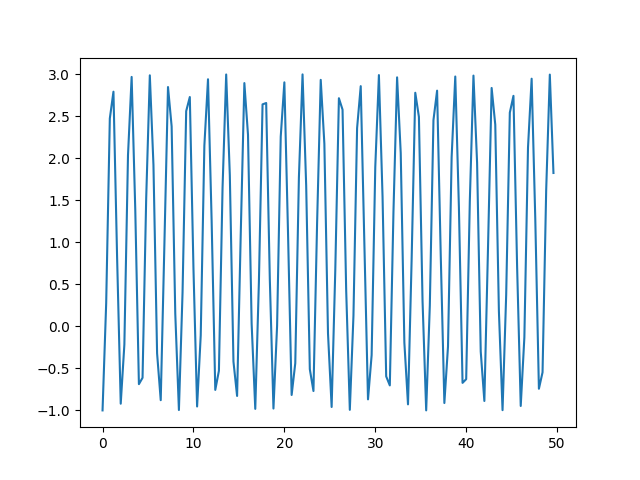
\includegraphics[width=\linewidth]{cgp/cosines_original}
			\caption{original cosine plot}
			\endminipage \hfill
			\minipage{0.32\textwidth}
			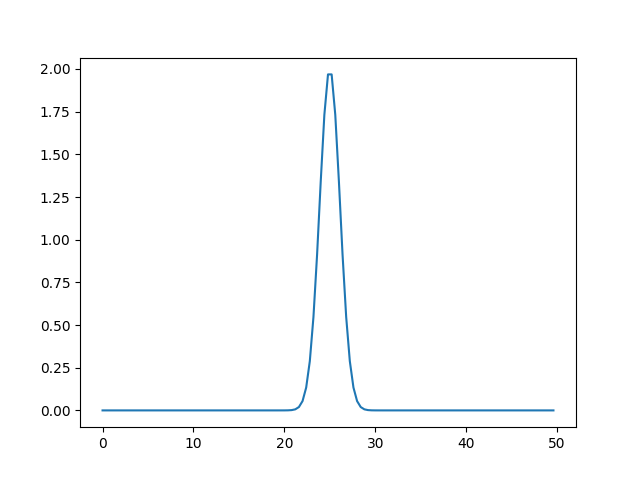
\includegraphics[width=\linewidth]{cgp/gauss_original}
			\caption{original gaussian plot}
			\endminipage \hfill
		\end{figure}
		\begin{figure}[H]
			\minipage{0.32\textwidth}
			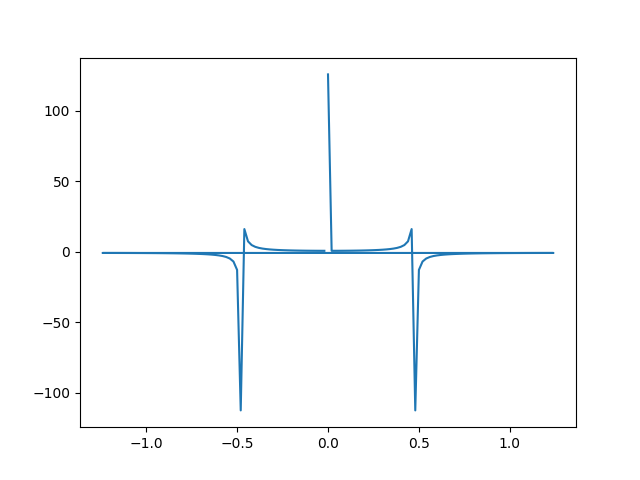
\includegraphics[width=\linewidth]{cgp/cosines_fft}
			\caption{fft cosine plot}
			\endminipage \hfill
			\minipage{0.32\textwidth}
			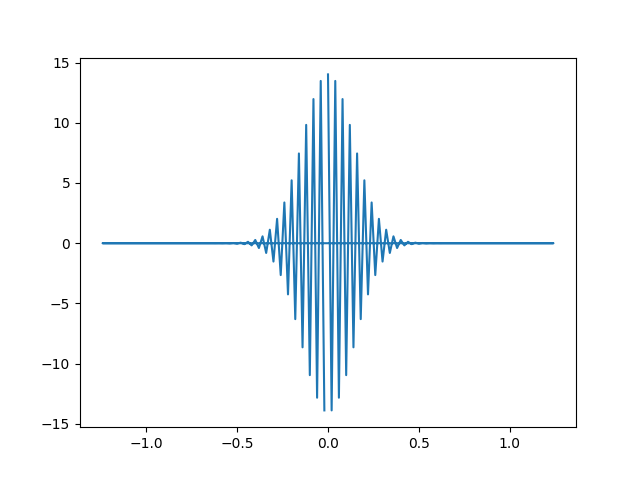
\includegraphics[width=\linewidth]{cgp/gauss_fft}
			\caption{fft gaussian plot}
			\endminipage \hfill
		\end{figure}
			
		\begin{figure}[H]
			\minipage{0.32\textwidth}
			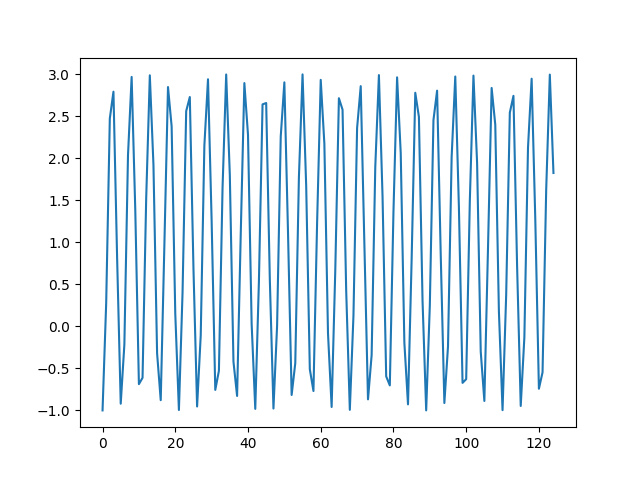
\includegraphics[width=\linewidth]{cgp/cosines_inverse_fft}
			\caption{inverse fft cosine plot}
			\endminipage \hfill
			\minipage{0.32\textwidth}
			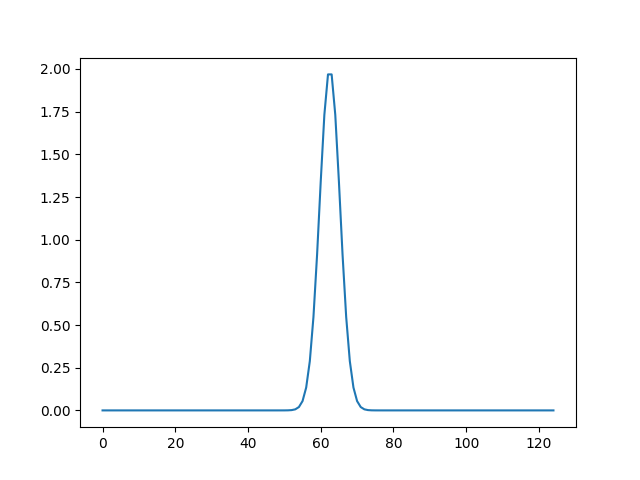
\includegraphics[width=\linewidth]{cgp/gauss_inverse_fft}
			\caption{inverse fft gaussian plot}
			\endminipage \hfill
		\end{figure}
		
		\par We can see that we recover the same plot at the beginning and at the end. The tighter the original gaussian was, the more rounded the fft peak. 
		
		
	\end{enumerate}
	\item 
	\begin{enumerate}
	\begin{figure}[H]
		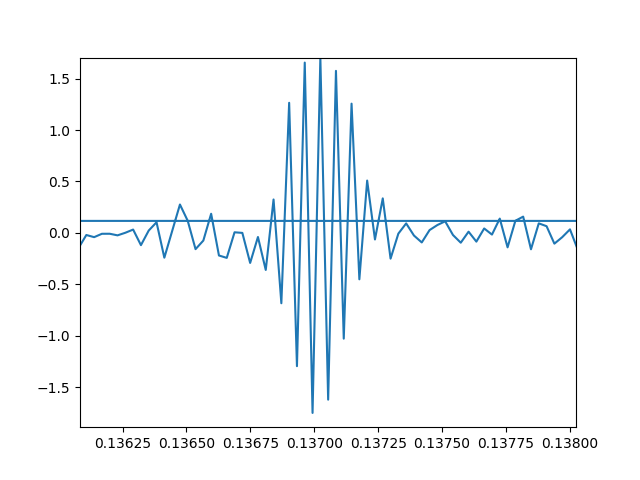
\includegraphics[width=\linewidth]{ap/peak}
		\caption{Arescibo peak}
	\end{figure}
		\item  According to the plot above, the peak frequency is around 0.137 cycles/ms; since the x axis is shifted down 1420 MHz, the peak is at 1420 MHz + 137 kHz. The signal is pretty round, suggesting that the original data was pointed. 
	\begin{figure}[H]
		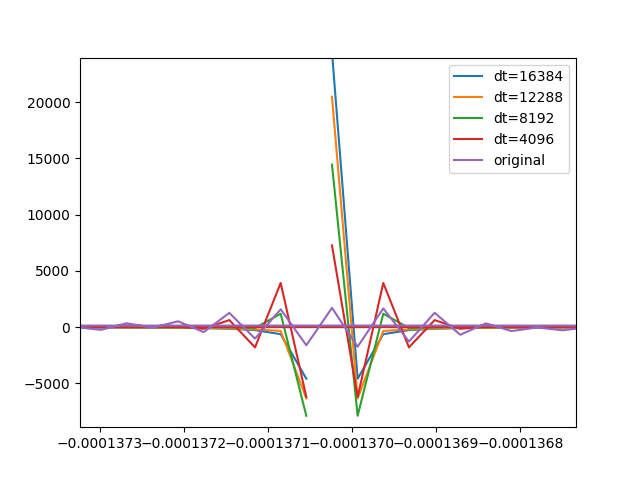
\includegraphics[width=\linewidth]{ap/dt}
		\caption{Arescibo peak}
	\end{figure}
		\item Looking at the plot above, the best estimate for the time constant $\Delta t$ is 4096 ms. 
	\end{enumerate}
	\item 
	\begin{enumerate}
		\item (nothing to do)
		\item 
			\begin{figure}[H]
			\minipage{0.32\textwidth}
			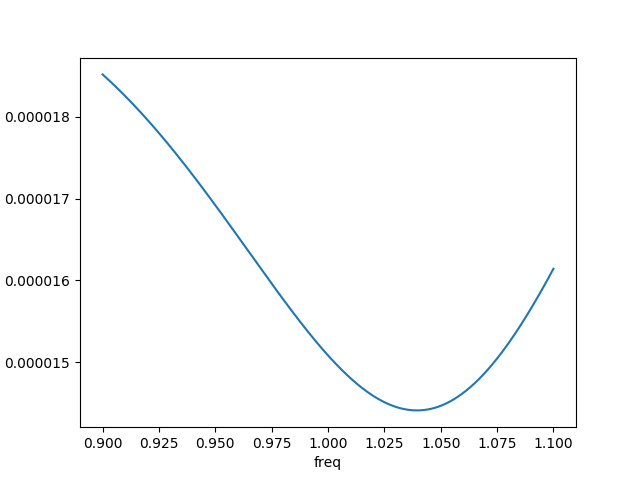
\includegraphics[width=\linewidth]{ls/gauss}
			\caption{lombscargle for evenly spaced gaussian}
			\endminipage \hfill
			\minipage{0.32\textwidth}
			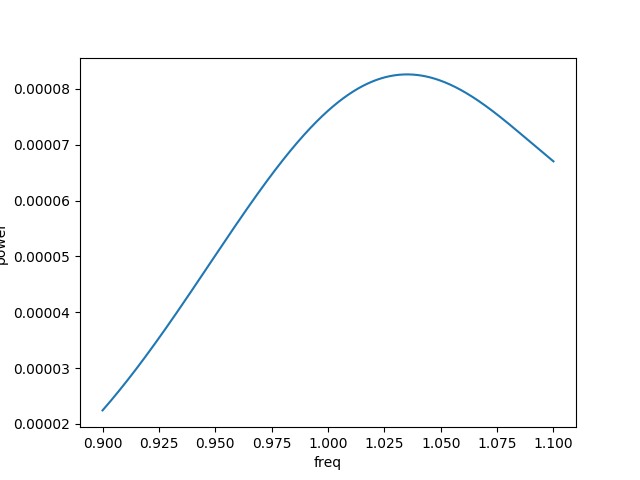
\includegraphics[width=\linewidth]{ls/arescibo}
			\caption{lombscargle for evenly spaced arescibo data}
			\endminipage \hfill
		\end{figure}
	\par These both give much less information than fft.
	
	\item 	
	\begin{figure}[H]
		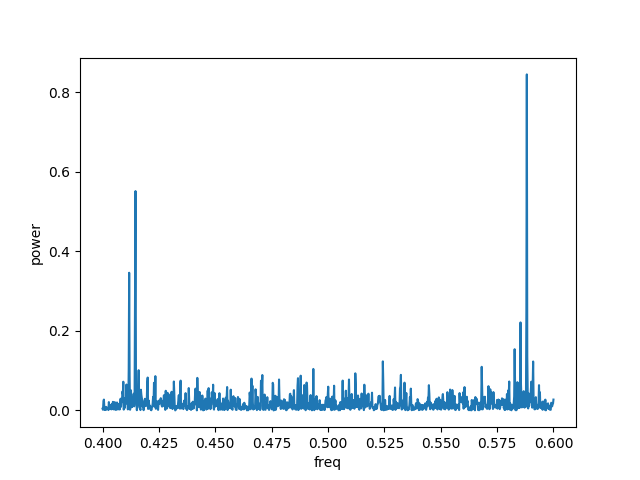
\includegraphics[width=\linewidth]{ls/uneven}
		\caption{Uneven HER-X1 data}
	\end{figure}
	\par We can see the peak at 1/1.7 = 0.5882; we can also see a secondary peak near 0.418, suggesting some other significant period of around 2.5 days. 
	\par Other significant frequencies could come from background noise in the observatory (radios, cellphones?).
	\end{enumerate}
\end{enumerate}


\end{document}
